\documentclass{article}

\usepackage{graphicx}
\usepackage{listings}

\begin{document}

\begin{center}


\includegraphics[width=3cm]{iiitb_comet_logo.jpg}

\vspace{0.4cm}

IIIT Bangalore

\vspace{0.3cm}

Name: Srinidhi A

ID: COMETFWC053

\vspace{0.5cm}

Question 59

\end{center}

\section*{Question}

Two push buttons $P_1$ and $P_2$ control the display of characters on a seven segment display.

Determine the logic expression for segment $g$.

\section*{Analysis}

The truth table for inputs $P_1$ and $P_2$ is

\begin{tabular}{c c c}
$P_1$ & $P_2$ & $g$ \\
0 & 0 & 0 \\
1 & 0 & 1 \\
0 & 1 & 1 \\
1 & 1 & 1 \\
\end{tabular}

From the table we observe that the segment turns ON when either $P_1$ or $P_2$ is 1.

Therefore the Boolean expression is

$g = P_1 + P_2$

\section*{Python Code}

\begin{lstlisting}
import numpy as np
import matplotlib.pyplot as plt

P1 = np.array([0,1,0,1])
P2 = np.array([0,0,1,1])

g = P1 | P2

print("P1 P2 g")

for i in range(4):
    print(P1[i], P2[i], g[i])

x = np.arange(4)

plt.step(x,P1,where='post',label='P1')
plt.step(x,P2,where='post',label='P2')
plt.step(x,g,where='post',label='g')

plt.grid()
plt.legend()

plt.savefig("graph.png")

plt.show()
\end{lstlisting}

\section*{Graph}

\begin{center}

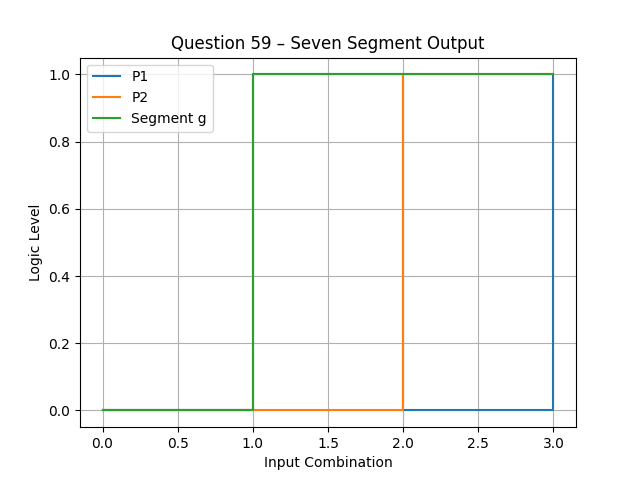
\includegraphics[width=10cm]{graph.png}

\end{center}

\section*{Conclusion}

The output follows the Boolean expression $g = P_1 + P_2$. The segment becomes active whenever either of the push buttons is pressed. The Python graph confirms the OR gate behavior.

\end{document}
